\chapter{Partie back-end}
\section{Introduction}

Le back-end est responsable de faire le lien entre les capteurs (qui nous fournissent les données en passant par le serveur LoRa de la partie "Infrastructure"), de traiter/normaliser les données et être capable de les fournir au front-end. De plus, le front-end doit être capable de changer l'intervalle de rafraîchissement du capteur.

\section{Technologies utilisées}

Les technologies utilisées sont les suivantes:

\begin{itemize}
\item[•] \href{https://nodejs.org/en/}{NodeJS} - Le coeur du système.
\item[•] \href{https://swagger.io/}{Swagger} - Permet de gérer les endpoints.
\item[•] \href{https://www.mongodb.com/}{MongoDB} - Permet de stocker les données de façon persistante.
\item[•] \href{https://www.docker.com}{Docker} - Pour gérer le déploiement
\end{itemize}

\section{Spécificités}

Voici l'infrastructure du back-end:

\begin{figure}[h!]
\centering
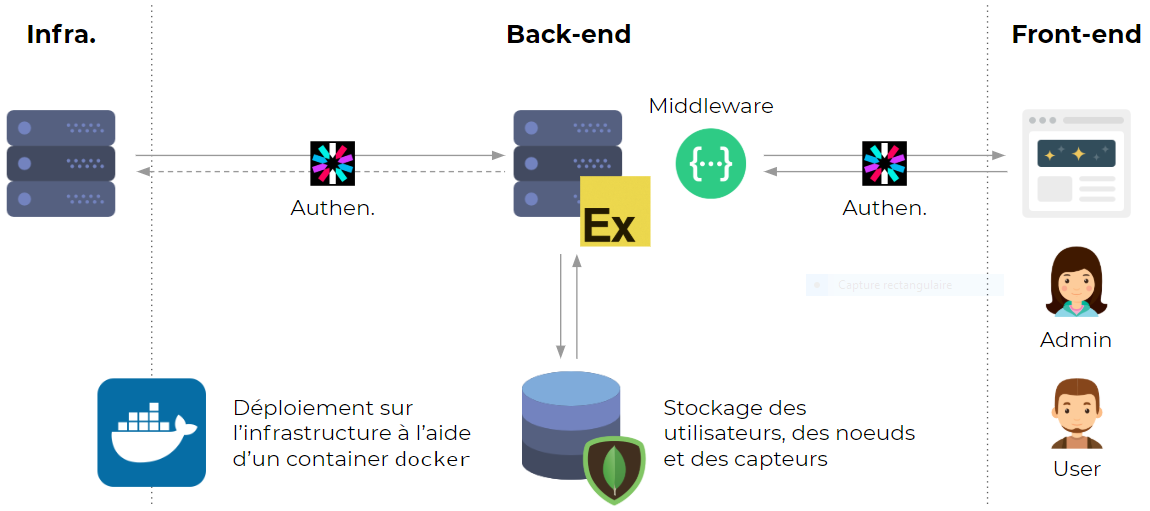
\includegraphics[width=\textwidth]{infra}
\caption{Infrastructure du back-end}
\end{figure}
    
\subsection{Contraintes}

Le back-end doit mettre à disposition une API permettant à un client de récupérer les informations des différents capteurs. Voici les différentes contraintes de ce dernier:

\begin{itemize}
\item[•] Le back-end doit savoir quel est le format envoyé de la part de chacun des capteurs.
\item[•] Le back-end doit pouvoir traiter et normaliser les données issues des capteurs.
\item[•] Le back-end doit pouvoir fournir les données des capteurs par noeuds (regroupement de plusieurs capteurs) ou par capteurs uniques.
\item[•] Le back-end doit pouvoir modifier le taux de rafraîchissement des capteurs.
\item[•] Le back-end doit permettre de pouvoir gérer des droits d'accès sur les endpoints.
\end{itemize}
   
\subsection{Authentification}
\label{ssec:be-auth}

Afin de garantir que seuls les utilisateurs autorisés puisse accéder/utiliser l'API, des \texttt{JSON Web Tokens (JWT)} seront utilisés et devront être utilisés lors des communications afin de savoir si un client est authentifié et autorisé à accéder à la ressource souhaitée.

\subsubsection{Obtenir un JWT}

Un JWT peut être obtenu en se connectant avec un nom d'utilisateur et un mot passe valide. Pour ce faire il faut effectuer une requête HTTP POST sur le endpoint \texttt{/auth}. En paramètre, dans le body de la requête, il faut fournir un payload json contenant les informations mentionnées ci-dessus.
\medskip

\begin{lstlisting}[style=Java]
{
    "username": "user",
    "password": "user1234"
}
\end{lstlisting}

Si l'utilisateur existe et que le mot de passe est valide, l'API REST retournera un réponse au format \texttt{text/plain} et le JWT généré se trouvera dans le body de la requête.

\subsubsection{Accéder à un endpoint protégé}

Pour accéder à un endpoint protégé, il faudra ajouter le header \texttt{Authorization} à vos requêtes avec comme valeur \texttt{Bearer <JWT>} ou \texttt{<JWT>} et à remplacer par le token récupéré à l'étape précédente.

Si l'utilisateur pour lequel ce JWT a été généré a les droit d'accès (autorisation) au endpoint au question, la requête sera authentifiée et autorisée. Les deux rôles existants sont \textbf{administrateur} ou \textbf{utilisateur} par défaut.

Pour plus de détails, notamment sur les contraintes de validation du payload, consulter la \href{https://github.com/heig-vd-iot2018/back-end/blob/master/dev/iot-rest-api/api/swagger/swagger.md}{spécification de l'API REST}.

\subsubsection{Utilisateurs existants par défaut}

Deux utilisateurs existants sont créés par défaut lors du déploiement de l'API sur un serveur. Par défaut et en mode développement ces utilisateurs sont:
\medskip

\renewcommand{\arraystretch}{1.2}
\begin{tabular}{|l|l|l|}
\hline
\textbf{Username} & \textbf{Password} & \textbf{Role} \\
\hline
user & user1234 & utilisateur par défaut \\
admin & admin1234 & administrateur \\
\hline
\end{tabular}
\renewcommand{\arraystretch}{1}
\medskip

Attention à ne pas garder ces mots de passes et noms d'utilisateurs lors du déploiement. Se référer à la section déploiement pour plus d'information.

\subsection{Représentations}

Les différents éléments du monde réels sont représentés de la façon suivante:

\begin{itemize}
\item[•] Un nœud est un regroupement de capteurs physiquement placés au même endroit.
\item[•] Un capteur comporte, à première vue, un capteur physique et le module de communication de LoRa.
\item[•]  Un capteur a un identifiant unique qui lui est associé et que l'on peut récupérer pour identifier précisément le capteur.
\end{itemize}

\subsection{Éléments stockés dans la base de données}

Deux principales collections seront stockés dans la base de donnée MongoDB:

\begin{itemize}
\item[•] La collection \texttt{Users} qui contiendra les utilisateurs autorisés à accéder à l'API. 
\begin{itemize}
\item[$\circ$] Dans le cadre de ce projet, chaque utilisateur sera stocké en dur.
\item[$\circ$] Lorsqu'un utilisateur est authentifié, il se verra attribuer un identifiant unique qu'il devra utiliser à chaque communication avec le serveur qui l'autorisera à accéder aux endpoints. Voir le chapitre \hyperref[ssec:be-auth]{Authentification} pour plus de détails.
\item[$\circ$] La structure de l'objet est la suivante:
\begin{itemize}
\item[\tiny$\blacksquare$] \texttt{username} - Le nom de l'utilisateur
\item[\tiny$\blacksquare$] \texttt{password} - Le mot de passe (stocké de façon sécurisée)
\item[\tiny$\blacksquare$] \texttt{role} - le rôle (lié aux droits d'accès de l'utilisateur) [0: utilisateur normal | 1: administrateur]
\end{itemize}
\end{itemize}
\medskip

\item[•] La collection \texttt{BlacklistedTokens} qui contiendra les tokens qui ne sont plus autorisés à accéder à l'API. 
\begin{itemize}
\item[$\circ$] Dans le cadre de ce projet, cette collection ne sera pas nettoyée automatiquement.
\item[$\circ$] La structure de l'objet est la suivante: 
\begin{itemize}
\item[\tiny$\blacksquare$] \texttt{blacklisted\_token} - Le token banni.
\end{itemize}
\end{itemize}
\clearpage

\item[•] La collection \texttt{Sensors} qui contiendra toutes les descriptions des différents capteurs. 
\begin{itemize}
\item[$\circ$] La structure de l'objet est la suivante: 
\begin{itemize}
\item[\tiny$\blacksquare$] \texttt{id} - Identifiant unique du capteur (récupéré par le LoRa serveur).
\item[\tiny$\blacksquare$] \texttt{documentationLink} - Lien vers la documentation officielle du constructeur.
\item[\tiny$\blacksquare$] \texttt{dateCreated} - La date à laquelle l'objet a été créé.
\item[\tiny$\blacksquare$] \texttt{dateUpdated} - La dernière date de mise à jour de l'objet.
\item[\tiny$\blacksquare$] \texttt{active} - Permet de savoir si le capteur est encore actif ou s'il a été désactivé.
\item[\tiny$\blacksquare$] \texttt{refresh\_interval} - Fréquence à laquelle le capteur doit fournir ses mesures.
\end{itemize}
\end{itemize}
\vspace{5mm}

\item[•] La collection \texttt{Nodes} qui contiendra toutes les descriptions des différents capteurs situés aux même endroit. 
\begin{itemize}
\item[$\circ$] La structure de l'objet est la suivante: 
\begin{itemize}
\item[\tiny$\blacksquare$] \texttt{id} - Identifiant unique du noeud.
\item[\tiny$\blacksquare$] \texttt{dateCreated} - La date à laquelle l'objet a été créé.
\item[\tiny$\blacksquare$] \texttt{dateUpdated} - La dernière date de mise à jour de l'objet.
\item[\tiny$\blacksquare$] \texttt{active} - Permet de savoir si le noeud est encore actif ou s'il a été désactivé.
\item[\tiny$\blacksquare$] \texttt{latitude} - La latitude du noeud.
\item[\tiny$\blacksquare$] \texttt{longitude} - La longitude du noeud.
\item[\tiny$\blacksquare$] \texttt{sensors} - Tableau d'entiers correspondant aux identifiants des capteurs regroupés dans le noeud.
\end{itemize}
\end{itemize}
\end{itemize}

\subsection{Endpoints}

Les différents endpoints et leurs définitions sont décrits \href{https://github.com/heig-vd-iot2018/back-end/blob/master/dev/iot-rest-api/api/swagger/swagger.md}{ici} et sont générés à l'aide du module \href{https://www.npmjs.com/package/swagger-markdown}{\texttt{NPM swagger-markdown}}.

La définition des endpoints sera régulièrement mise à jour.   
\clearpage

\section{Déploiement}

Pour le déploiement, une configuration \texttt{Docker} a été créée. Les instructions sont disponibles \href{https://github.com/heig-vd-iot2018/back-end/blob/master/dev/README.md}{ici}.

\section{Conclusion}

Le back-end a réussi à être connecté au front-end. Des données mock-up ont été créées pour permettre au front-end d'afficher des données même si la connexion au serveur LoRa n'est pas une réussite que nous ne parvenons pas à obtenir des informations en provenance de vrais capteurs.
   
\section{Documentation supplémentaire}

Toutes les librairies utilisées pour ce projet sont disponibles dans le \href{https://github.com/heig-vd-iot2018/back-end/blob/master/dev/iot-rest-api/package.json}{\texttt{package.json}}.
\clearpage